\chapter{Oscillation} \label{ch:oscillation}
This chapter investigates the qualitative similarity between finite population 
short-term behavior and infinite population evolutionary limits predicted by Vose. 
It uses computation to verify predicted infinite population limits and presents 
necessary and sufficient conditions for convergence to periodic orbits. 
We compute mutation distribution $\bm{\mu}$ and crossover distribution $\bm{\chi}$ 
to satisfy those conditions. Through experiments, we explore our second research 
question: can finite populations exhibit oscillation behavior in practice?

\section{Limits}
\label{Limits}
Vose states that under mild assumptions on mutation (explained later), infinite populations converge under repeated application 
of $\mathcal{M}$ in the absense of selective pressure. Vose mentions that periodic orbits are possible, but populations converge under 
repeated application of $\mathcal{M}^2$ and the limits $\bm{p}^\ast = \lim_{n \rightarrow \infty} \mathcal{M}^{2n}({\bm p})$ 
and ${\bm q}^\ast = \lim_{n \rightarrow \infty} \mathcal{M}^{2n+1}({\bm q})$ exist (see \cite{Vose1999}).

Following Vose (see \cite{Vose1999}), let $S_g = g \mathcal{R} \setminus \{\textbf{0}, g\}$, and let $|g|$ be the number of non zero bits in $g$. 
If $\widehat{\bm{p}}$ represents the current population in Walsh coordinates, then the next generation ${\widehat{\bm{p}}_g}^{\prime}$ 
(expressed in Walsh coordinates) is 
\[
{{\widehat{\bm{p}}}_g}^{\prime}  = \begin{cases}
    2^{\ell /2}  & \text{if $g = 0$}\\
    x_g \widehat{{\bm p}}_g + y_g(\widehat{{\bm p}}_g) & \text{otherwise}
  \end{cases}
\]
where
\[
x_g = 2\widehat{\mathcal{M}}_{g,0},  \hspace*{1cm} y_g(z) = 2^{\ell /2} \sum_{i \in S_g} z_i z_{i+g} \widehat{\mathcal{M}}_{i,i+g}.
\]

Moreover, 
\begin{eqnarray*}
|g| \;=\; 1 \nudge & \Longrightarrow & y_g = 0 \\
|g| \;>\; 0 \nudge & \Longrightarrow & |x_g| \leq 1 \\
|x_g| \;=\; 1 \nudge & \Longrightarrow & y_g = 0
\end{eqnarray*}

With above notations, the limits can be expressed in the Walsh basis by recursive equations (see \cite{Vose1999})
\begin{equation}
\label{lt1}
\widehat{{\bm p}^{\ast}}_g  = \begin{cases}
    (x_g y_g(\widehat{{\bm p}^{\ast}}) + y_g(\widehat{{\bm q}^{\ast}}))/(1-x_g^2)  & \text{if $|x_g| < 0$}\\
    \widehat{p}_g  & \text{otherwise}
  \end{cases}
\end{equation}
\begin{equation}
\label{lt2}
\widehat{{\bm q}^{\ast}}_g  = \begin{cases}
    (x_g y_g(\widehat{{\bm q}^{\ast}}) + y_g(\widehat{{\bm p}^{\ast}}))/(1-x_g^2)  & \text{if $|x_g| < 0$}\\
    \widehat{\mathcal{M}({\bm p})_g}  & \text{otherwise}
  \end{cases}
\end{equation}

If $x_g \neq -1$ for all $g$, then ${\bm p}^\ast = {\bm q}^\ast = \lim_{n \rightarrow \infty} \mathcal{M}({\bm p})$ is the limit of mixing. In other cases, 
mixing converges to a periodic orbit oscillating between ${\bm p}^\ast$ and ${\bm q}^\ast = \mathcal{M}({\bm p}^\ast)$.

Limits $\widehat{{\bm p}^{\ast}}_g$ and $\widehat{{\bm q}^{\ast}_g}$ can be computed considering $g$th components in order of increasing $|g|$.
The necessary and sufficient condition for the sequence
\[
\bm{p}, \mathcal{M}({\bm p}), \mathcal{M}^2({\bm p}),\cdots
\]
to converge to a periodic orbit is that for some $g$
\begin{equation}
\label{OscCond}
-1 = \sum \limits_{j} (-1)^{g^T j} \bm{\mu}_j = - \sum \limits_{k \in \bar{g}\mathcal{R}} \bm{\chi}_{k+g} + \bm{\chi}_k
\end{equation}
 
\section{Mutation and Crossover Distributions}
The following describes the generation of mutation and crossover distributions that satisfy equation \ref{OscCond} 
for evolution to converge to a periodic orbit. 
Let $\bm{\mu}$ and $\bm{\chi}$ represent mutation and crossover distributions (respectively), 
and let $U01()$ return a random number between $0$ and $1$. For any $g \in \mathcal{R}$, $g \neq 0$, and for all $j \in \mathcal{R}$,
\begin{equation}
\label{MuDist}
\bm{\mu}_j = \begin{cases}
    U01() & \text{if $g^T j$ is odd}\\
    0 & \text{otherwise}
  \end{cases}
\end{equation}

Normalization yields $\bm{\mu}$ (the mutation distribution),
\[
\bm{\mu}_j := \bm{\mu}_j / \sum \limits_{j \in \mathcal{R} } \bm{\mu}_j.
\]
Moreover, $\bm{\mu}$ satisfies condition \ref{OscCond}.

Condition $k \in \bar{g} \mathcal{R}$ in equation \ref{OscCond} is
\[
k = \bar{g} i  \text{ for some $i \in \mathcal{R}$}
\]
Multiplying through by $\bar{g}$ yields
\begin{equation*}
\bar{g} k = \bar{g} \bar{g} i \; = \; \bar{g} i \; = \; k 
\end{equation*}
The crossover distribution can therefore be generated as follows.
For all $k \in \mathcal{R}$,
\begin{equation}
\label{ChiDist}
\begin{split}
\bm{\chi}_k & \;=\;  U01() \;\; \mbox{if}\; \bar{g}k \;=\; k \\
\bm{\chi}_{k+g} & \;=\;  U01() \;\; \mbox{if}\; \bar{g}k \;=\; k\\
\bm{\chi}_k & \;=\;  0  \;\; otherwise.
\end{split}
\end{equation} 
Normalization yields 
$\bm{\chi}$ (the crossover distribution),
\[
\bm{\chi}_k := \bm{\chi}_k/\sum\limits_{k \in \mathcal{R}} \bm{\chi}_k.
\]
Moreover, $\bm{\chi}_k$ satisfies condition \ref{OscCond}.

\section{Initial Population}
\label{InitPopOsc}

% \begin{figure}[H]
% \begin{center}
% \resizebox*{12cm}{!}{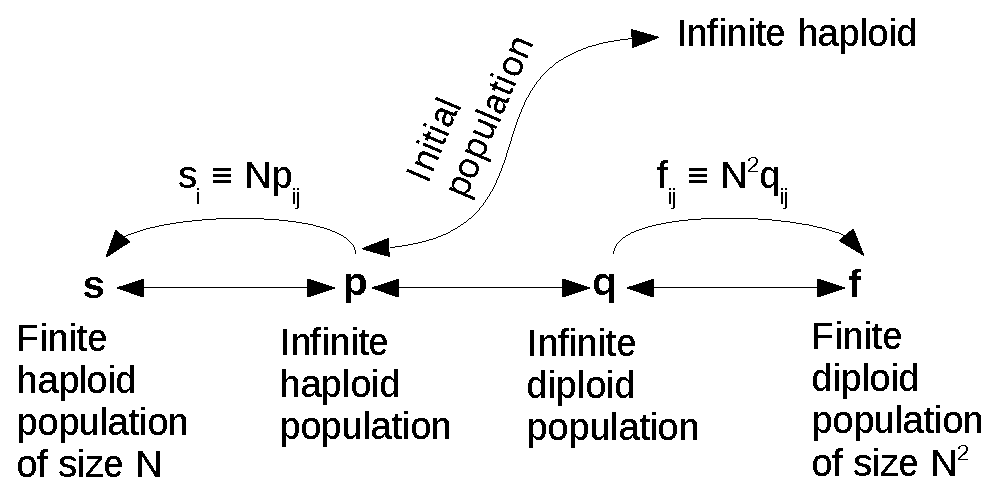
\includegraphics{figures/eps/initialpop.eps}}\hspace{4pt}
% \caption{\textbf{Initial population computation} }
% \label{initialpop}
% \end{center}
% \end{figure}
% Let finite haploid population $\bm{s}^n$, finite diploid population $\bm{f}^n$, infinite haploid population $\bm{p}^n$ 
% and infinite haploid population $\bm{q}^n$ be considered with initial population $\bm{s}^0$, $\bm{f}^0$,
% $\bm{p}^0$, $\bm{q}^0$ respectively. 
To investigate oscillation in infinite population and finite population behavior, 
it is desirable to have the same or corresponding initial populations. 

For string length $\ell$, the number of possible haploids is $x = 2^\ell$. Let array $\bm{t}$ represent a  
population of size $N$ as follows: $\bm{t}_j$ is the $j$th population member (some element of $\{0,..,x-1\}$ 
where elements are base 2 length $\ell$ binary strings). Array $\bm{t}$ is generated from a random vector $\bm{u}$ of size $x$ as follows. 
\begin{eqnarray*}
\bm{u}_i & = & U01(); \tabspace {i = 0,.., x-1} \\
\bm{t}_j & = & randp(\bm{u}) ; \tabspace {j = 0,.., N-1}
\end{eqnarray*}
where $randp(\bm{u})$ returns random index $i$ into array $\bm{u}$ with probability $\bm{u}_i$.

Let $\bm{c}_i$ be the count of haploid member $i$ in population $\bm{t}$,
\[
\bm{c}_i = \sum \limits_{j=0}^{N-1} [\bm{t}_j = i]  \nudge; \tabspace  {i = 0,.., x-1}
\]
The infinite population vector $\bm{p}$ has $i$th component
\[
\bm{p}_i = \frac{\bm{c}_i}{ N }.
\]
This randomly generated infinite haploid population vector $\bm{p}$ is used to obtain a diploid infinite population vector $\bm{q}$,  
and finite population vectors $\bm{s}$ and $\bm{f}$ as follows.

Infinite diploid population $\bm{q}$ is calculated corresponding to initial haploid population $\bm{p}$ as
\[
\bm{q}_{i,j} = \bm{p}_i \bm{p}_j  \nudge; \tabspace  (0 \leq i,j < x)
\]

The finite haploid population members are the elements of array $\bm{t}$, 
the corresponding finite haploid population vector $\bm{s}$ is identical to $\bm{p}$. 
Let $\bm{v}$ be a finite diploid population member array of dimension two and of size $N^2$ whose diploid member 
$\bm{v}[i][j]$ at index $[i][j]$ is
\[
\bm{v}[i][j] \;=\; \langle \bm{t}_i, \bm{t}_j \rangle \tabspace 0 \leq i,j < N
\]
The finite diploid population (proportion) vector $\bm{f}$ corresponding to 
finite diploid population member array $\bm{v}$ is identical to $\bm{q}$.
% \[
% \bm{c}_i = N \cdot \bm{p}_i 
% \]
% \[
% \sum \limits_{j=0}^{N-1} [\bm{t}_j = i] = \bm{c}_i  \nudge; \tabspace  {i = 0,.., x-1} 
% \]

Thus, initial infinite haploid population vector $\bm{p}$ corresponds to initial infinite diploid 
population vector $\bm{q}$, and to initial finite 
haploid population vector $\bm{s}$ with population size $N$ and population member array $\bm{t}$, 
and to initial finite diploid population vector $\bm{f}$ with population size $N^2$ and population member array $\bm{v}$.

\section{Oscillation}
\label{Oscillation}

Crossover distribution $\bm{\chi}$ and mutation distribution $\bm{\mu}$ satisfying 
condition (\ref{OscCond}) are considered to investigate oscillating behavior near 
predicted infinite population evolutionary limits.

Infinite haploid population evolutionary limits $\bm{p}_h^{\ast}$ and $\bm{q}_h^{\ast}$ 
were computed using equations (\ref{lt1}) and (\ref{lt2}). 
Infinite diploid population evolutionary limits $\bm{p}_d^{\ast}$ and $\bm{q}_d^{\ast}$ are obtained as follows
\begin{eqnarray*}
({\bm{p}_d^{\ast}})_{\langle \gamma_0, \gamma_1 \rangle} & = & ({\bm{p}_h^{\ast}})_{\gamma_0} ({\bm{p}_h^{\ast}})_{\gamma_1} \\
({\bm{q}_d^{\ast}})_{\langle \gamma_0, \gamma_1 \rangle} & = & ({\bm{q}_h^{\ast}})_{\gamma_0} ({\bm{q}_h^{\ast}})_{\gamma_1}
\end{eqnarray*}
where $\gamma = \langle \gamma_0, \gamma_1 \rangle$ is a diploid genome.

For every genome length $\ell$, the same initial population (calculated as described in (\ref{InitPopOsc})) was used for the infinite population and all 
sizes of finite populations conisdered.
Genome lengths $\ell \in \{8, \nudge10, \nudge12, \nudge14\}$ were used. Base population size of $N_0 = 64$ was used 
for the finite haploid case to compute initial population vector. The population sizes considered for plotting 
graphs were $N \in \{N_0^2, \nudge10N_0^2, \nudge20N_0^2\}$. 
To study oscillation in finite populations, the distances of $\bm{p}^n$ and $\bm{s}^n$ to haploid evolutionary limits $\bm{p}_h^{\ast}$ and 
$\bm{q}_h^{\ast}$ were plotted and the distances of $\bm{q}^n$ and 
$\bm{f}^n$ to diploid evolutionary limits $\bm{p}_d^{\ast}$ and $\bm{q}_d^{\ast}$ were plotted. 

According to the results and conclusions from 
chapter 2, the expected distance $d$ between finite population of size $N$ and infinite population is 
\[
d \approx 1/\sqrt{N}
\]
\begin{table}[H]
\caption{\textbf{Expected single step distance $d$ for population size $N$}}
\centering
\begin{tabular}{c c c c}
\hline
$N$ & 4096 & 40960 & 81920 \\
$d$ & 0.0156 & 0.0049 & 0.0035 \\
\hline
\end{tabular}
\label{tableExpectedDistance}
\end{table}
The distance between finite population and infinite population, for both haploid and diploid cases, were also plotted. 
%oscillation
% haploids
\subsection{Haploid Population}

% l = 8
\begin{figure}[h]
\begin{center}
\subfloat{
\resizebox{8cm}{4.5cm}{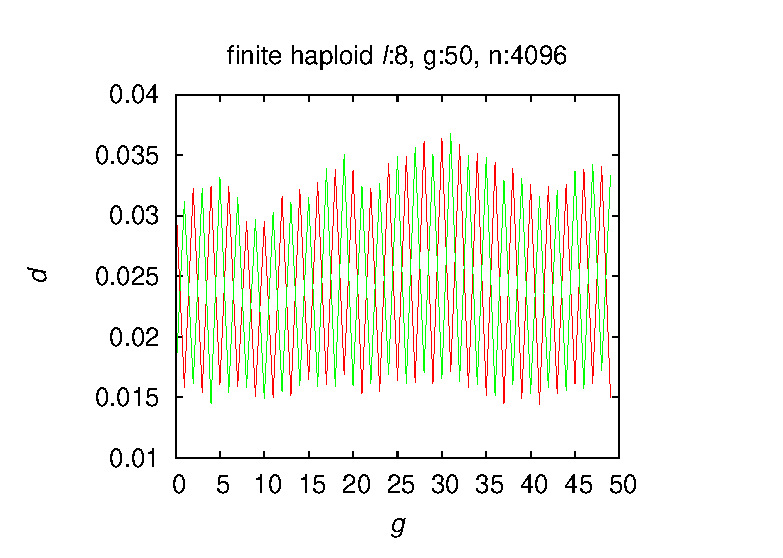
\includegraphics{figures/eps/osc/b8/n004096_osc_fin_hap.eps}}} \hspace{-3em}% 
\subfloat{
\resizebox{8cm}{4.5cm}{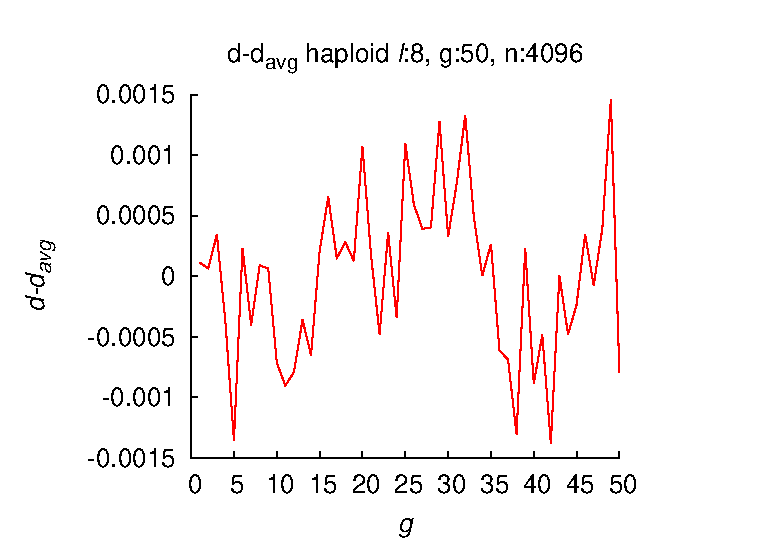
\includegraphics{figures/eps/osc/b8/n004096_osc_fin_hap_dist.eps}}} \vspace{-1em}  \hspace{-3em}% 

\end{center}
\begin{center}
\subfloat{
\resizebox{8cm}{4.5cm}{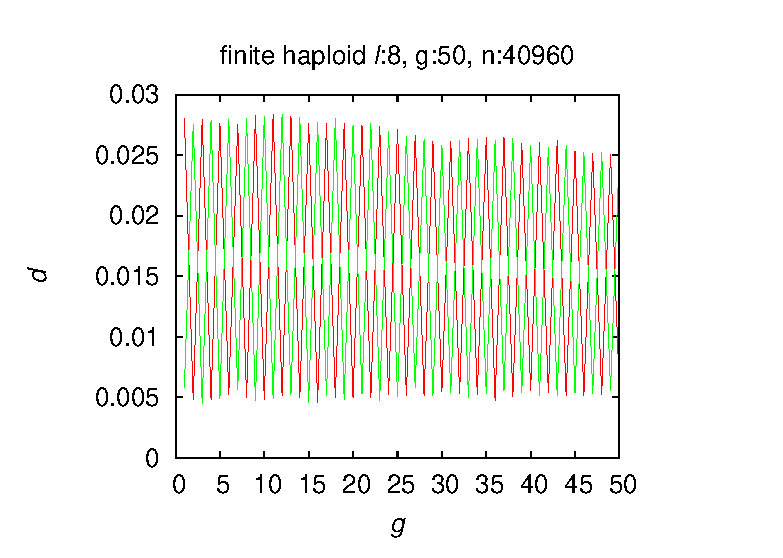
\includegraphics{figures/eps/osc/b8/n040960_osc_fin_hap.eps}}} \hspace{-3em}% 
\subfloat{
\resizebox{8cm}{4.5cm}{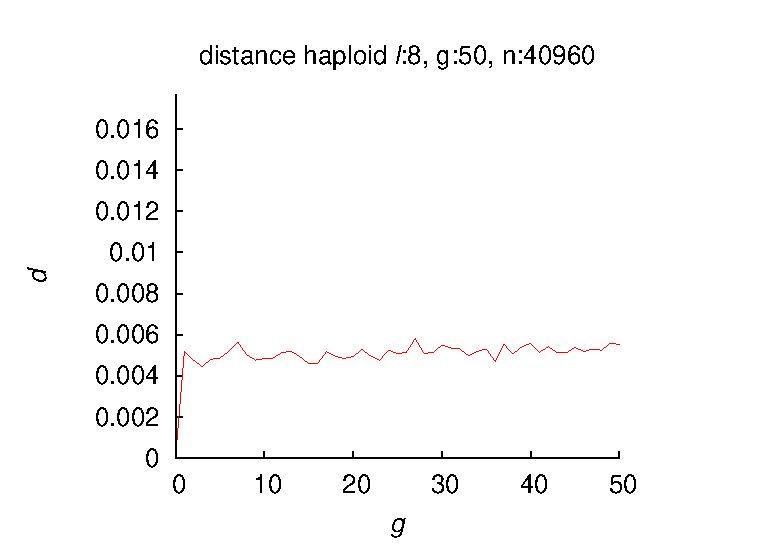
\includegraphics{figures/eps/osc/b8/n040960_osc_fin_hap_dist.eps}}} \vspace{-1em}  \hspace{-3em}% 
\end{center}
\end{figure}

\begin{figure}[h]
\begin{center}
\subfloat{
\resizebox{8cm}{4.5cm}{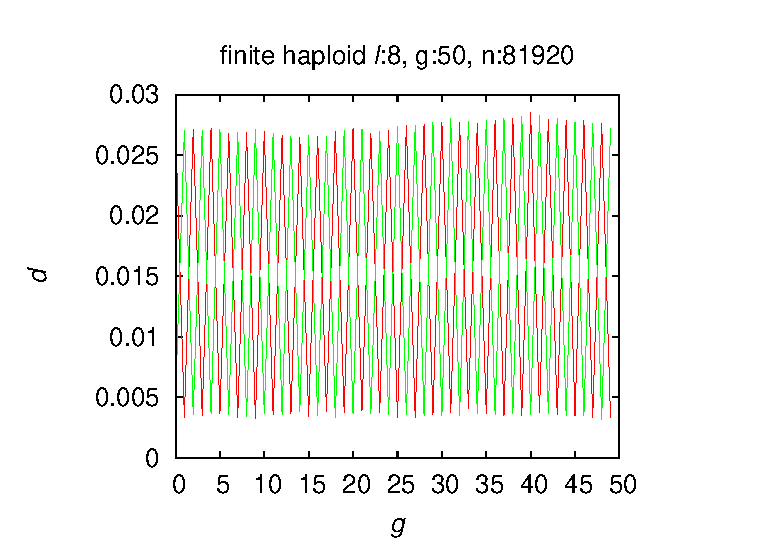
\includegraphics{figures/eps/osc/b8/n081920_osc_fin_hap.eps}}} \hspace{-3em}% 
\subfloat{
\resizebox{8cm}{4.5cm}{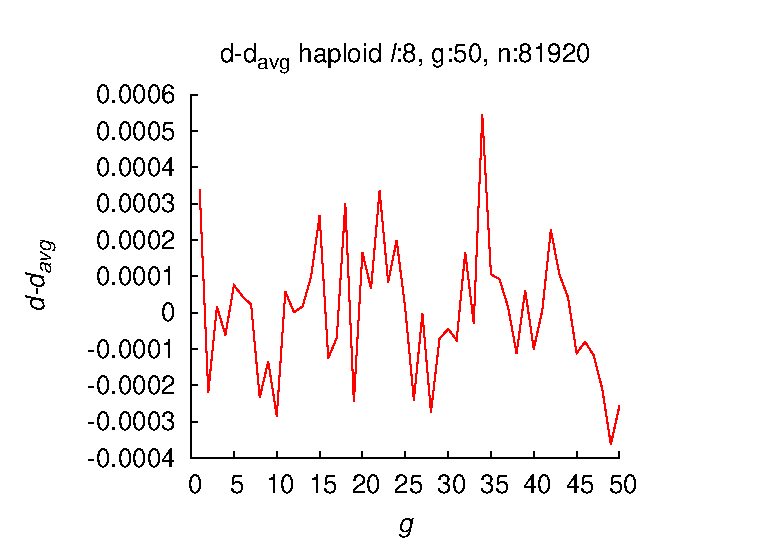
\includegraphics{figures/eps/osc/b8/n081920_osc_fin_hap_dist.eps}}} \vspace{-1em}  \hspace{-3em}% 
\end{center}


\begin{center}
\subfloat{
\resizebox{8cm}{4.5cm}{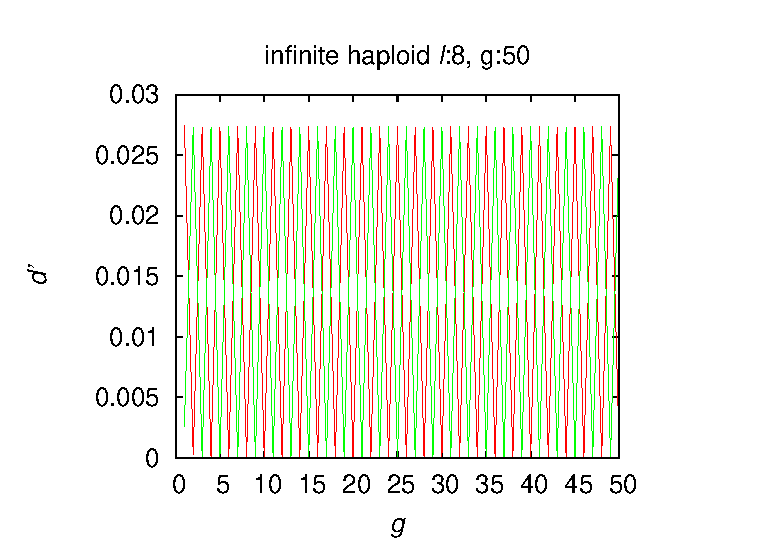
\includegraphics{figures/eps/osc/b8/osc_inf_hap.eps}}} \hspace{-3em}%
\subfloat{
\resizebox{8cm}{4.5cm}{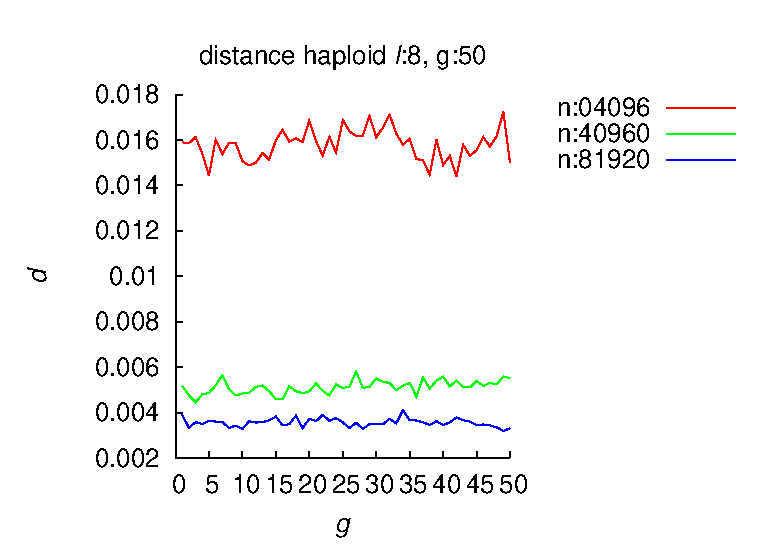
\includegraphics{figures/eps/osc/b8/fin_hap_dist.eps}}} \vspace{-0.5em} \hspace{-3em}%

\caption[\textbf{Infinite and finite haploid population oscillation behavior for genome length $\ell = 8$}]{\textbf{Infinite and finite haploid population oscillation behavior for genome length $\ell = 8$:} In left column, $d'$ is
  distance of finite population of size $n$ or infinite population to limits for $g$ generations. In right column, $d$ is 
  distance of finite population to infinite population for $g$ generations and $d_{avg}$ is average distance.}
\label{oscillation_8h}
\end{center}
\end{figure}

% l = 10

\begin{figure}[h]

\begin{center}
\subfloat{
\resizebox{8cm}{4.5cm}{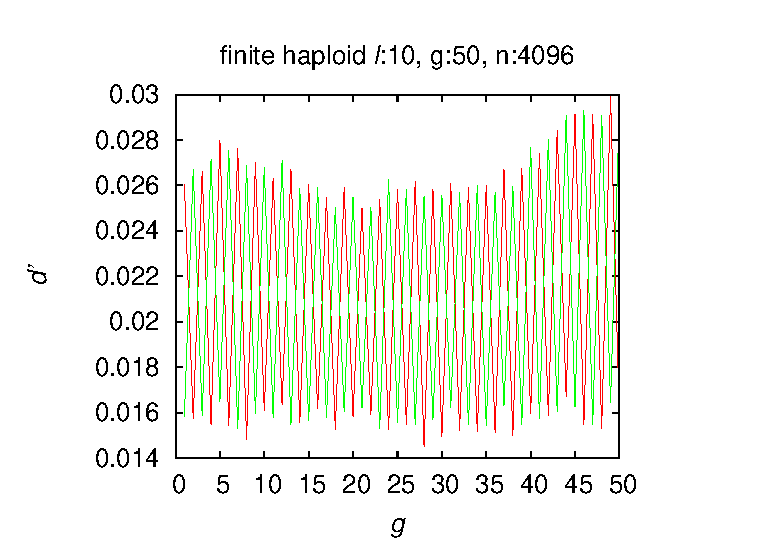
\includegraphics{figures/eps/osc/b10/n004096_osc_fin_hap.eps}}} \hspace{-3em}% 
\subfloat{
\resizebox{8cm}{4.5cm}{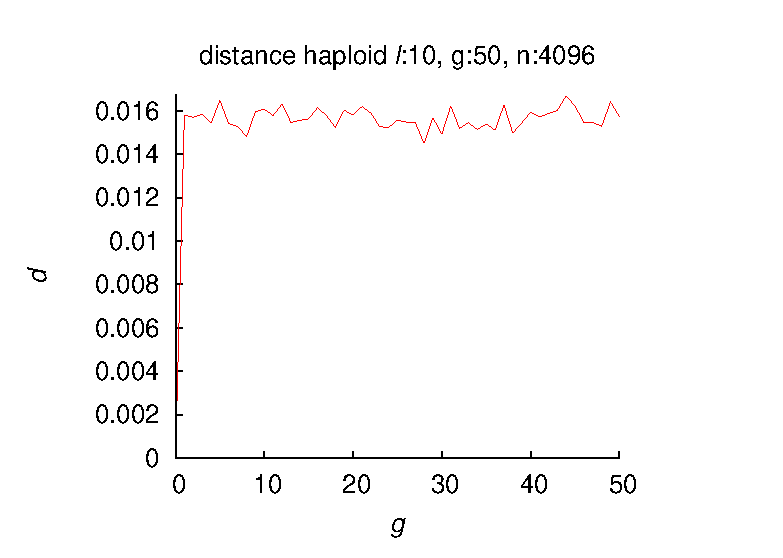
\includegraphics{figures/eps/osc/b10/n004096_osc_fin_hap_dist.eps}}} \vspace{-1em}  \hspace{-3em}% 
\end{center}
\begin{center}
\subfloat{
\resizebox{8cm}{4.5cm}{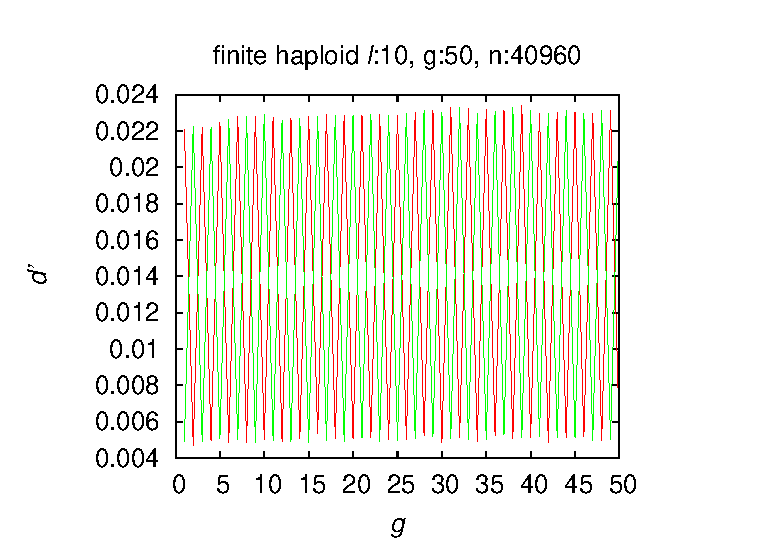
\includegraphics{figures/eps/osc/b10/n040960_osc_fin_hap.eps}}} \hspace{-3em}% 
\subfloat{
\resizebox{8cm}{4.5cm}{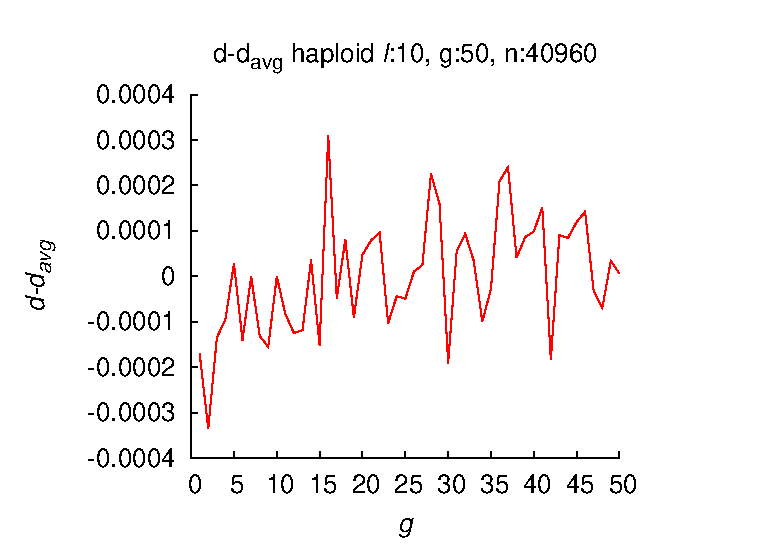
\includegraphics{figures/eps/osc/b10/n040960_osc_fin_hap_dist.eps}}} \vspace{-1em}  \hspace{-3em}% 
\end{center}

\begin{center}
\subfloat{
\resizebox{8cm}{4.5cm}{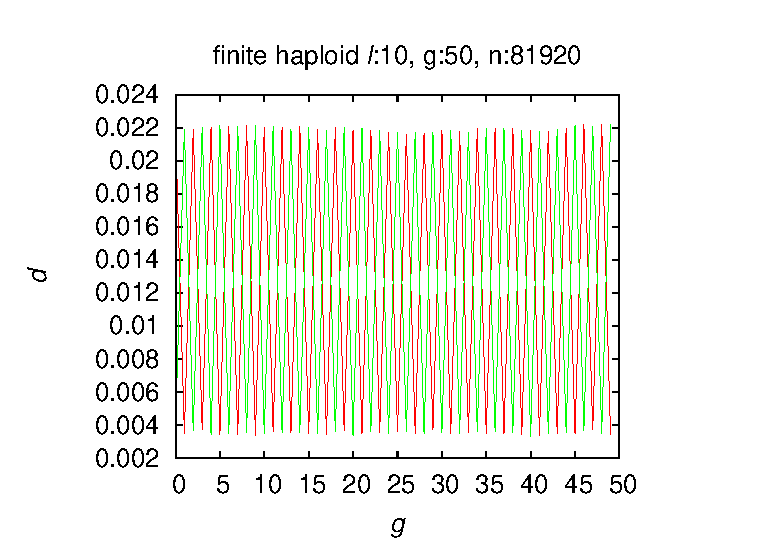
\includegraphics{figures/eps/osc/b10/n081920_osc_fin_hap.eps}}} \hspace{-3em}% 
\subfloat{
\resizebox{8cm}{4.5cm}{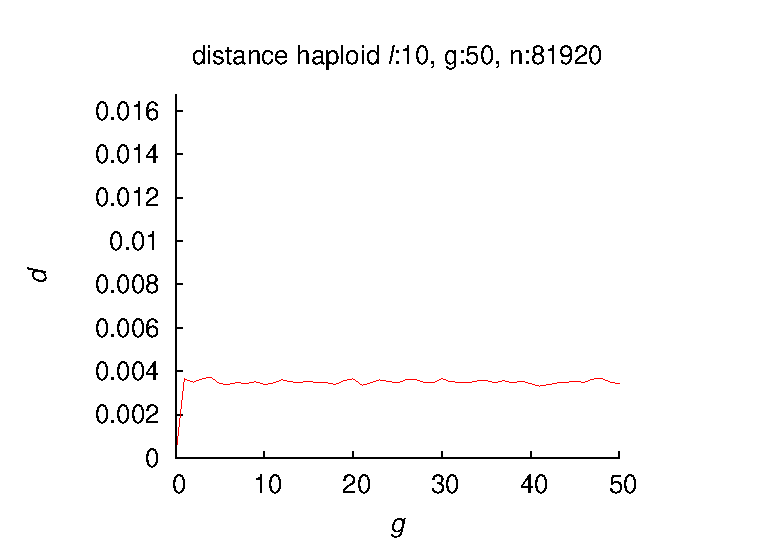
\includegraphics{figures/eps/osc/b10/n081920_osc_fin_hap_dist.eps}}} \vspace{-1em}  \hspace{-3em}% 
\end{center}

\begin{center}
\subfloat{
\resizebox{8cm}{4.5cm}{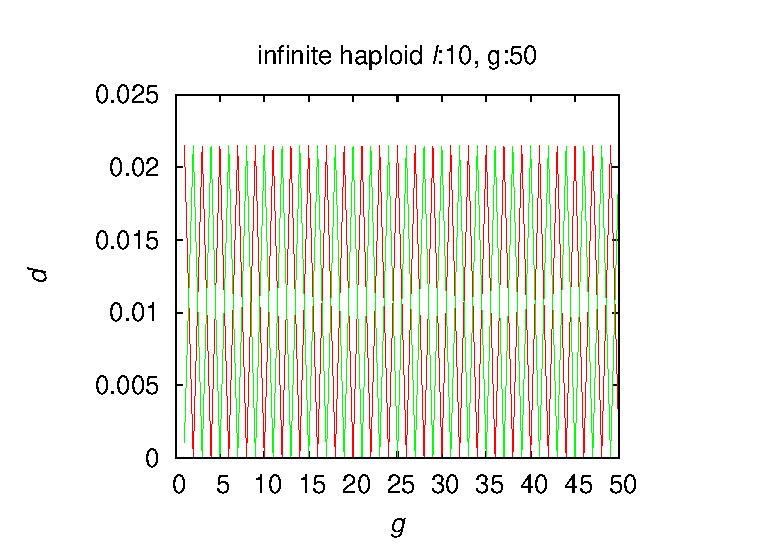
\includegraphics{figures/eps/osc/b10/osc_inf_hap.eps}}} \hspace{-3em}%
\subfloat{
\resizebox{8cm}{4.5cm}{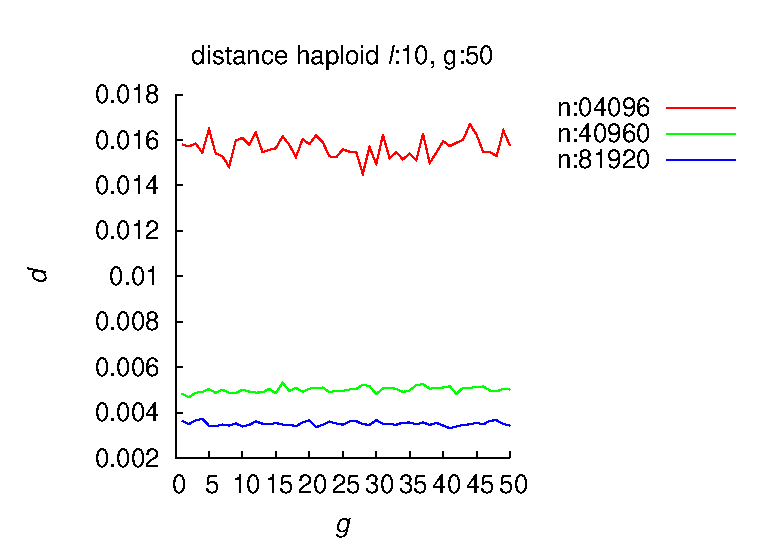
\includegraphics{figures/eps/osc/b10/fin_hap_dist.eps}}} \vspace{-0.5em} \hspace{-3em}%

\caption[\textbf{Infinite and finite haploid population oscillation behavior for genome length $\ell = 10$}]{\textbf{Infinite and finite haploid population oscillation behavior for genome length $\ell = 10$ :} In left column, $d'$ is
  distance of finite population of size $n$ or infinite population to limits for $g$ generations. In right column, $d$ is 
  distance of finite population to infinite population for $g$ generations and $d_{avg}$ is average distance.}
\label{oscillation_10h}
\end{center}
\end{figure}

% l = 12

\begin{figure}[h]

\begin{center}
\subfloat{
\resizebox{8cm}{4.5cm}{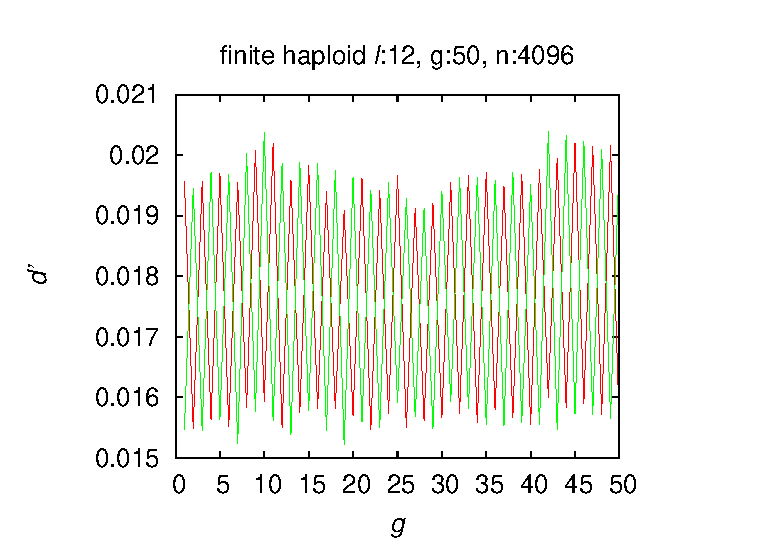
\includegraphics{figures/eps/osc/b12/n004096_osc_fin_hap.eps}}} \hspace{-3em}% 
\subfloat{
\resizebox{8cm}{4.5cm}{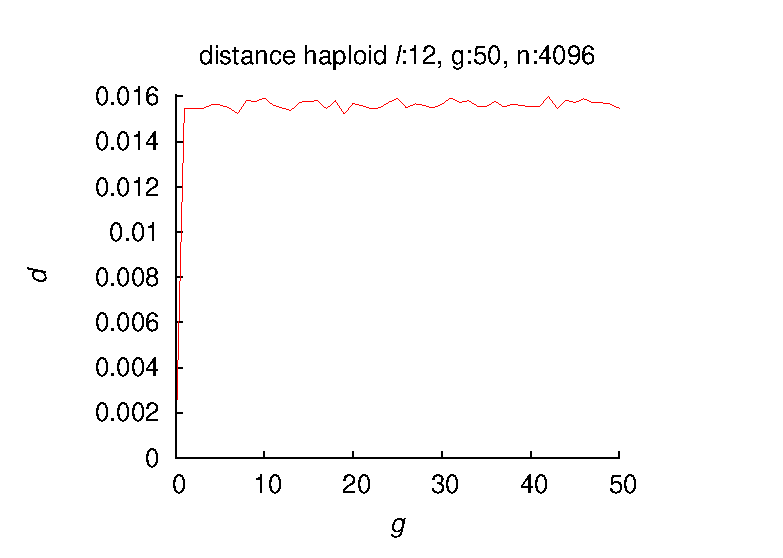
\includegraphics{figures/eps/osc/b12/n004096_osc_fin_hap_dist.eps}}} \vspace{-1em}  \hspace{-3em}% 
\end{center}
\begin{center}
\subfloat{
\resizebox{8cm}{4.5cm}{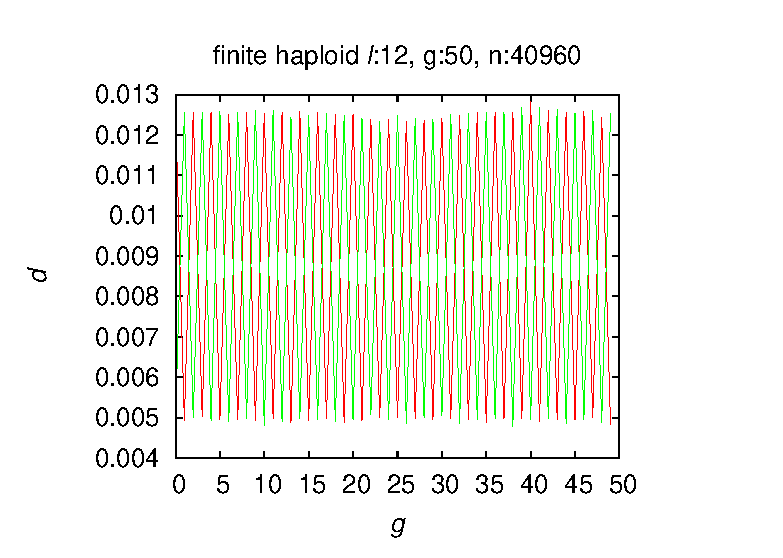
\includegraphics{figures/eps/osc/b12/n040960_osc_fin_hap.eps}}} \hspace{-3em}% 
\subfloat{
\resizebox{8cm}{4.5cm}{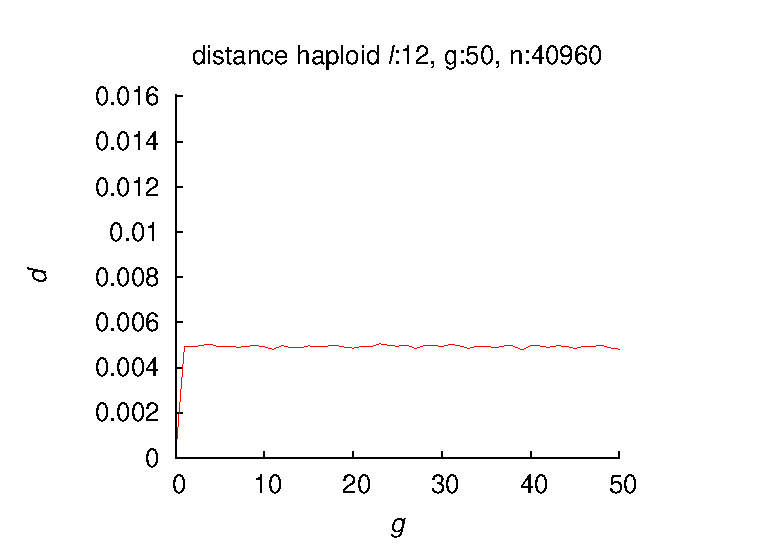
\includegraphics{figures/eps/osc/b12/n040960_osc_fin_hap_dist.eps}}} \vspace{-1em}  \hspace{-3em}% 
\end{center}
\begin{center}
\subfloat{
\resizebox{8cm}{4.5cm}{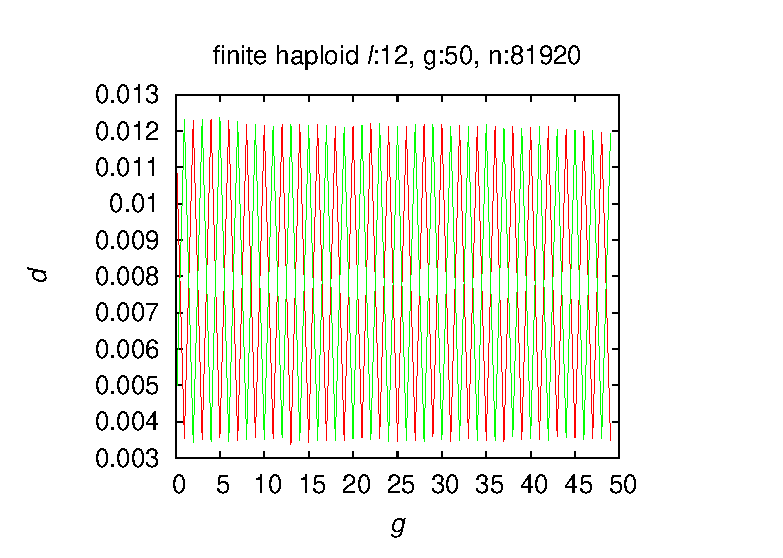
\includegraphics{figures/eps/osc/b12/n081920_osc_fin_hap.eps}}} \hspace{-3em}% 
\subfloat{
\resizebox{8cm}{4.5cm}{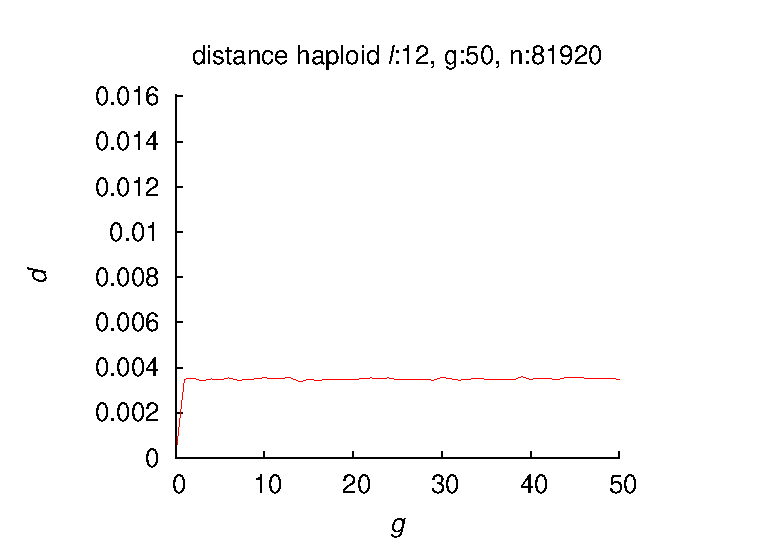
\includegraphics{figures/eps/osc/b12/n081920_osc_fin_hap_dist.eps}}} \vspace{-1em}  \hspace{-3em}% 
\end{center}

\begin{center}
\subfloat{
\resizebox{8cm}{4.5cm}{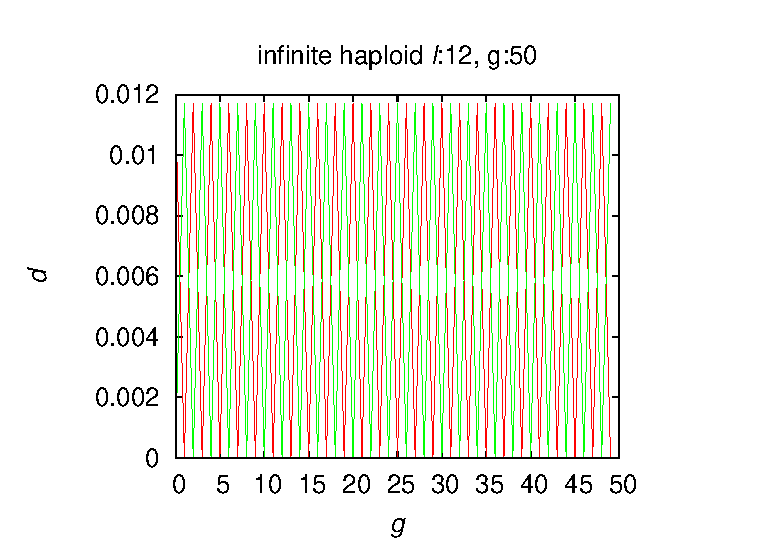
\includegraphics{figures/eps/osc/b12/osc_inf_hap.eps}}} \hspace{-3em}%
\subfloat{
\resizebox{8cm}{4.5cm}{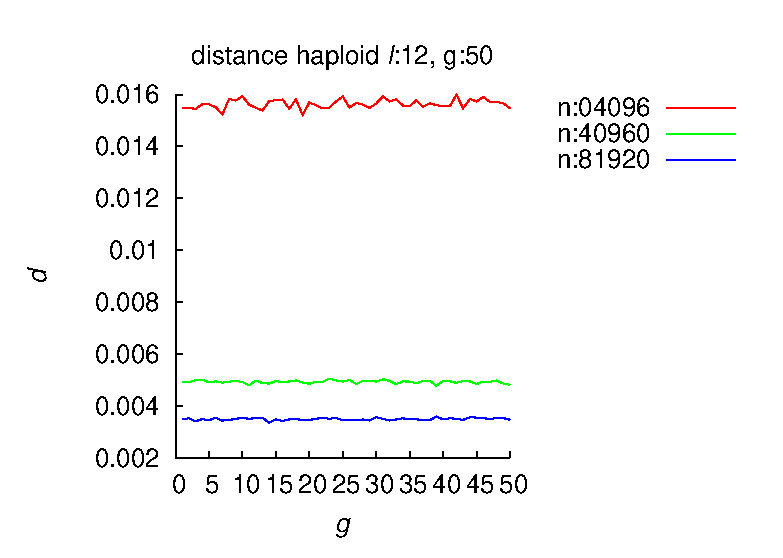
\includegraphics{figures/eps/osc/b12/fin_hap_dist.eps}}} \vspace{-0.5em} \hspace{-3em}%

\caption[\textbf{Infinite and finite haploid population oscillation behavior for genome length $\ell = 12$}]{\textbf{Infinite and finite haploid population oscillation behavior for genome length $\ell = 12$ :} In left column, $d'$ is
  distance of finite population of size $n$ or infinite population to limits for $g$ generations. In right column, $d$ is 
  distance of finite population to infinite population for $g$ generations and $d_{avg}$ is average distance.}
\label{oscillation_12h}
\end{center}
\end{figure}

% l= 14

\begin{figure}[h]

\begin{center}
\subfloat{
\resizebox{8cm}{4.5cm}{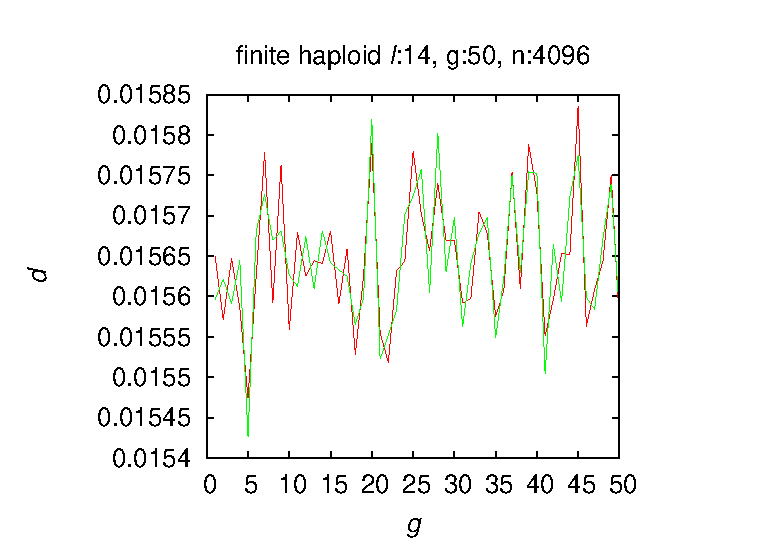
\includegraphics{figures/eps/osc/b14/n004096_osc_fin_hap.eps}}} \hspace{-3em}% 
\subfloat{
\resizebox{8cm}{4.5cm}{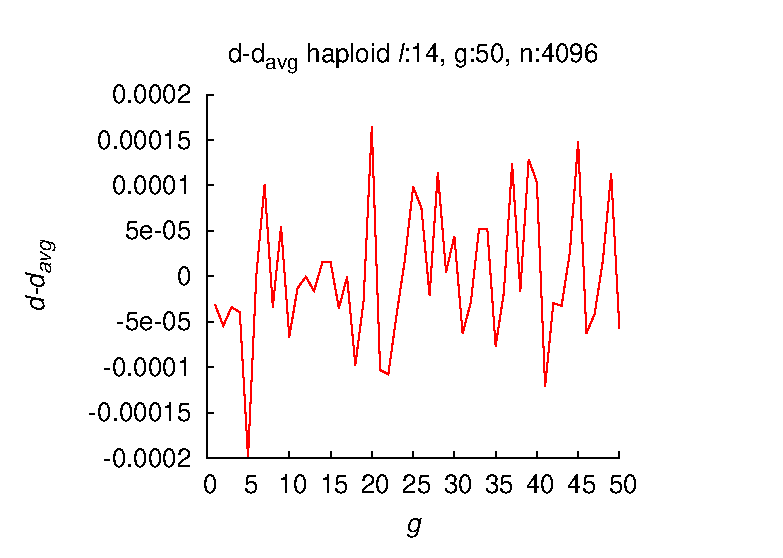
\includegraphics{figures/eps/osc/b14/n004096_osc_fin_hap_dist.eps}}} \vspace{-1em}  \hspace{-3em}% 
\end{center}
\begin{center}
\subfloat{
\resizebox{8cm}{4.5cm}{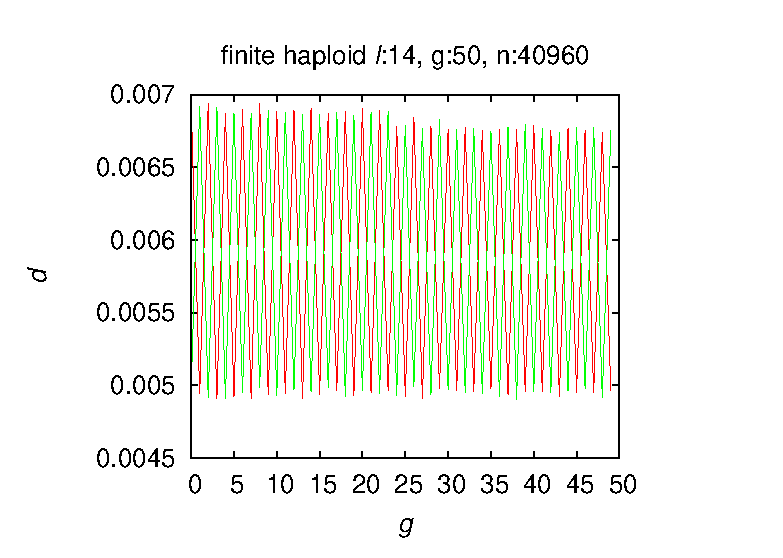
\includegraphics{figures/eps/osc/b14/n040960_osc_fin_hap.eps}}} \hspace{-3em}% 
\subfloat{
\resizebox{8cm}{4.5cm}{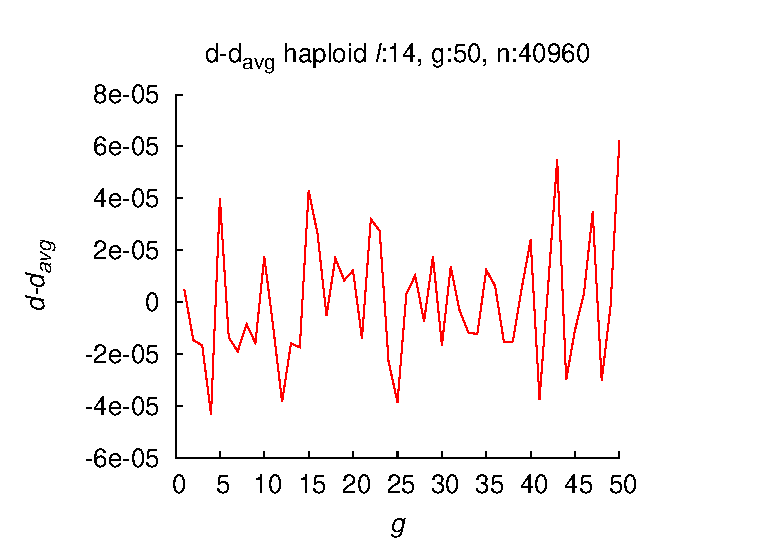
\includegraphics{figures/eps/osc/b14/n040960_osc_fin_hap_dist.eps}}} \vspace{-1em}  \hspace{-3em}% 
\end{center}

\begin{center}
\subfloat{
\resizebox{8cm}{4.5cm}{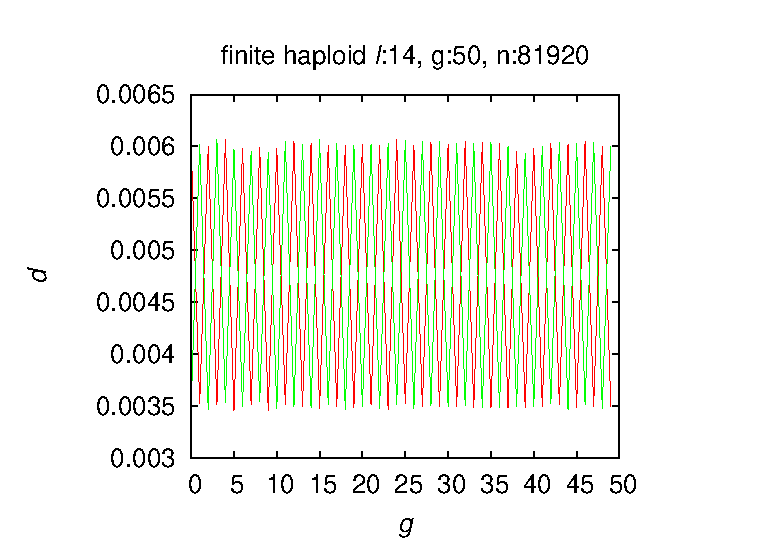
\includegraphics{figures/eps/osc/b14/n081920_osc_fin_hap.eps}}} \hspace{-3em}% 
\subfloat{
\resizebox{8cm}{4.5cm}{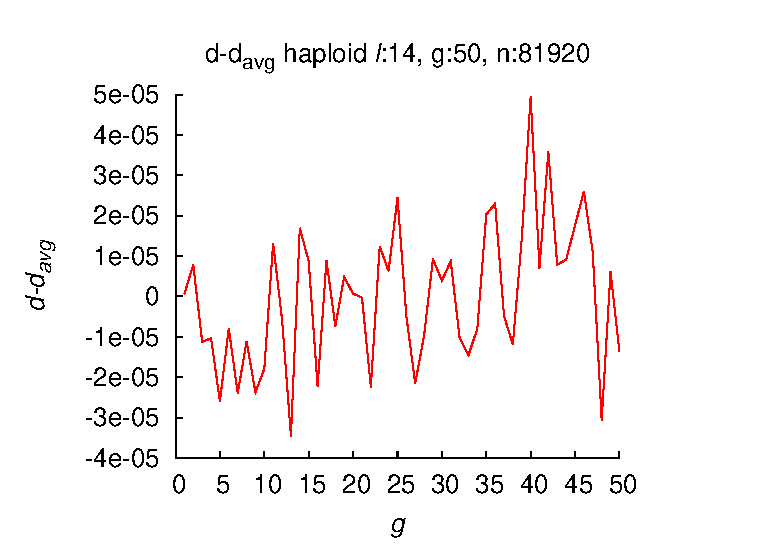
\includegraphics{figures/eps/osc/b14/n081920_osc_fin_hap_dist.eps}}} \vspace{-1em}  \hspace{-3em}% 
\end{center}

\begin{center}
\subfloat{
\resizebox{8cm}{4.5cm}{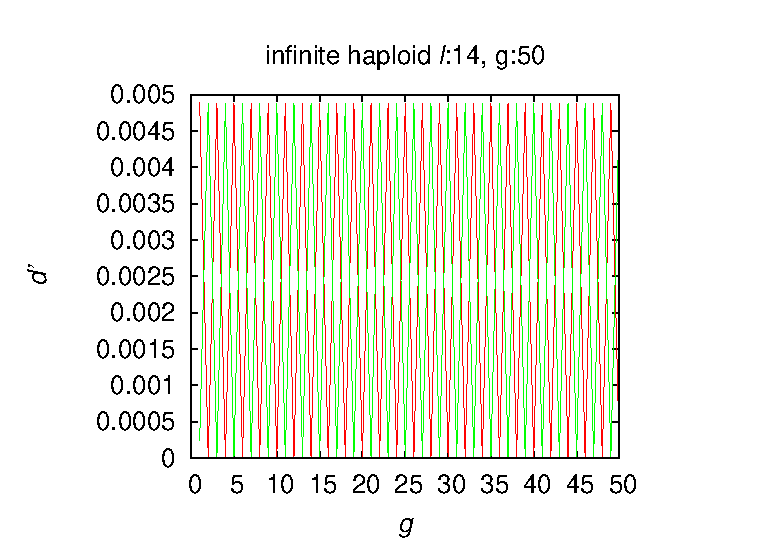
\includegraphics{figures/eps/osc/b14/osc_inf_hap.eps}}} \hspace{-3em}%
\subfloat{
\resizebox{8cm}{4.5cm}{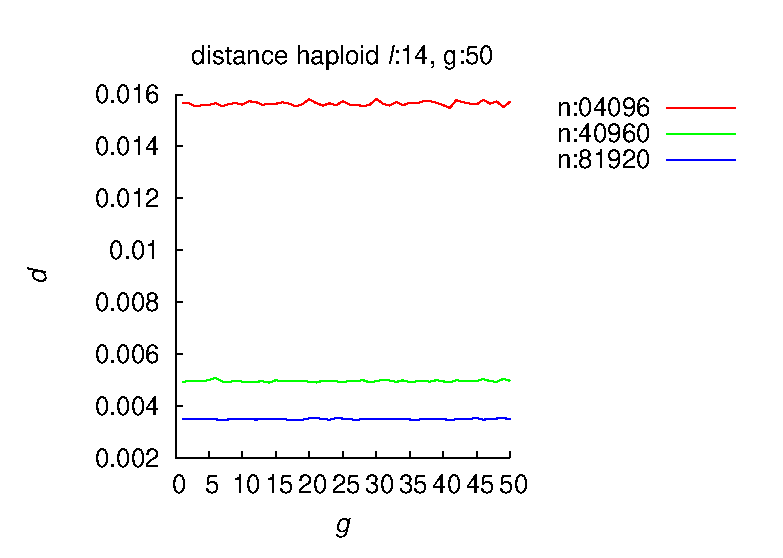
\includegraphics{figures/eps/osc/b14/fin_hap_dist.eps}}} \vspace{-0.5em} \hspace{-3em}%

\caption[\textbf{Infinite and finite haploid population oscillation behavior for genome length $\ell = 14$}]{\textbf{Infinite and finite haploid population oscillation behavior for genome length $\ell = 14$ :} In left column, $d'$ is
  distance of finite population of size $n$ or infinite population to limits for $g$ generations. In right column, $d$ is 
  distance of finite population to infinite population for $g$ generations and $d_{avg}$ is average distance.}
\label{oscillation_14h}
\end{center}
\end{figure}


\clearpage

\textbf{ Figures} \ref{oscillation_8h}, \ref{oscillation_10h}, \ref{oscillation_12h} and
\ref{oscillation_14h} show oscillations in finite haploid populations, and distances 
between finite haploid populations and infinite haploid populations arranged by genome length $\ell$ in ascending order. 
In each figure for unique genome length $\ell$, sub-figures 
are arranged by population size $N$. In each figure, the first three rows of sub-figures in the left column show distance $d'$ of finite population 
to limits, the sub-figure in fourth row of the left column shows distance $d'$ of infinite population to limits. These sub-figures depict 
oscillating behavior of both infinite and finite haploid populations when condition \ref{OscCond} is met. 
As population size increases, oscillation approaches the behavior exhibited by infinite population. 

In each figure (\ref{oscillation_8h}, \ref{oscillation_10h}, \ref{oscillation_12h}, 
and \ref{oscillation_14h}), the first three graphs in the right column show 
distance variation (difference of distance $d$ and average distance $d_{avg}$)  
where $d$ is distance between haploid finite and infinite populations and $d_{avg}$ is average value of $d$. 
The graph in the fourth row of the right column combines distance plots between finite and infinite populations for sizes 
($N = N_0^2, \nudge10N_0^2, \nudge20N_0^2$). The resulting graphs show distance decreases 
as population size increases, consistent with results from section \ref{convergence}. 
The graphs of $d-d_{avg}$ decrease in amplitude as population size increases. 
For fixed finite population size, as $\ell$ increases, the distance graphs become smoother, and amplitude of oscillations decrease. 

Distance data obtained from simulations for haploid populations are summarized in table \ref{tableDistanceOscHap},  
which tabulates average distance between finite and infinite populations 
for population sizes $N \;=\; 4096 $, $N \;=\; 40960 $ and $N \;=\; 81920 $.
\begin{table}[h]
\caption[\textbf{Distance measured for haploid population}]{\textbf{Distance measured for haploid population:} $N$ is population size, $\ell$ is genome length, 
average distance between finite and infinite population is tabulated in the last three columns, and last row is expected single step distance.}
\centering
\begin{tabularx}{0.75\textwidth}{ c *{3}{X}}
\toprule
$\ell$ & $N \;=\; 4096 $ & $N \;=\; 40960 $ & $N \;=\; 81920 $\\
\midrule
8 & 0.0158 & 0.0051 & 0.0035 \\
10 & 0.0157 & 0.0050 & 0.0035 \\ 
12 & 0.0156 & 0.0049 & 0.0035 \\
14 & 0.0156 & 0.0049 & 0.0035 \\ 
\midrule
$1/\sqrt{N}$ & 0.0156 & 0.0049 & 0.0035 \\
\bottomrule
\end{tabularx}
\label{tableDistanceOscHap}
\end{table}

Results from table \ref{tableDistanceOscHap} show average distance between finite and infinite population closely follows 
the expected single step distance. The distance decreases as $1/\sqrt{N}$.

\clearpage
% diploids
\subsection{Diploid Population}

% l = 8
\begin{figure}[h]

\begin{center}
\subfloat{
\resizebox{8cm}{4.5cm}{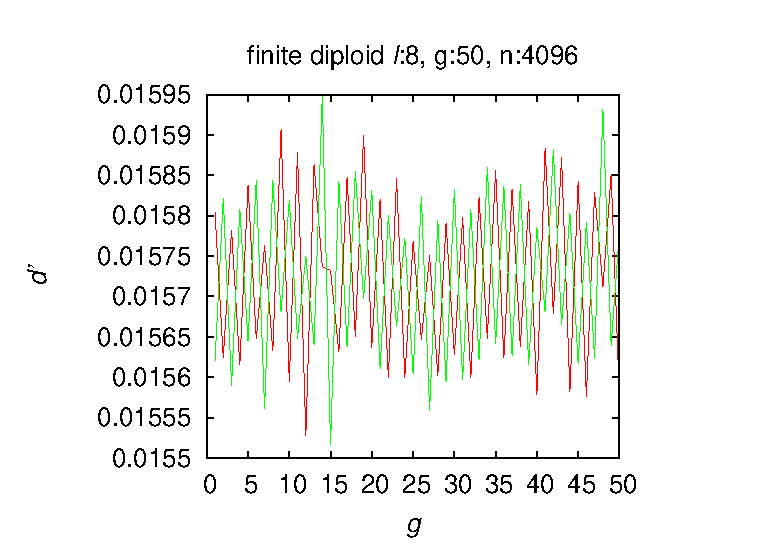
\includegraphics{figures/eps/osc/b8/n004096_osc_fin_dip.eps}}} \hspace{-3em}% 
\subfloat{
\resizebox{8cm}{4.5cm}{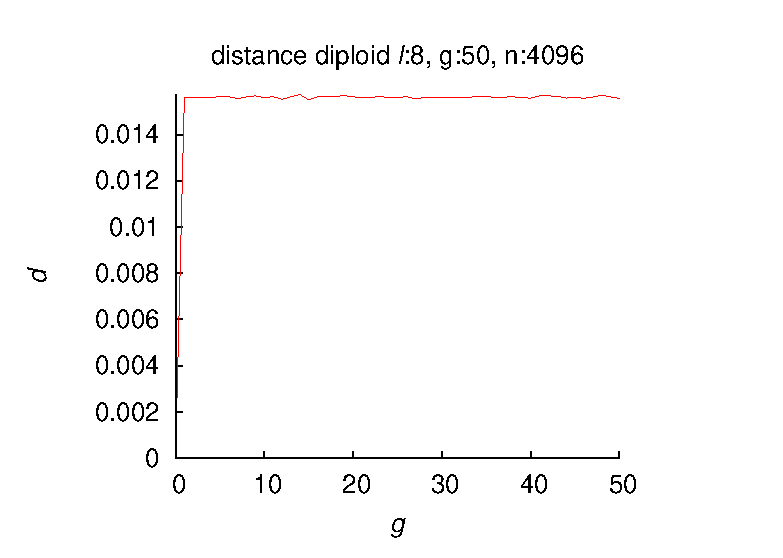
\includegraphics{figures/eps/osc/b8/n004096_osc_fin_dip_dist.eps}}}  \vspace{-1em}  \hspace{-3em}% 
\end{center}
\begin{center}
\subfloat{
\resizebox{8cm}{4.5cm}{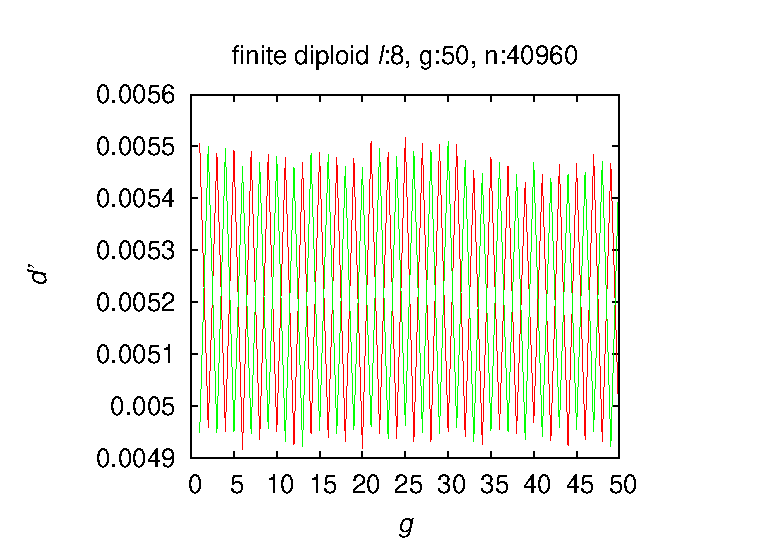
\includegraphics{figures/eps/osc/b8/n040960_osc_fin_dip.eps}}} \hspace{-3em}% 
\subfloat{
\resizebox{8cm}{4.5cm}{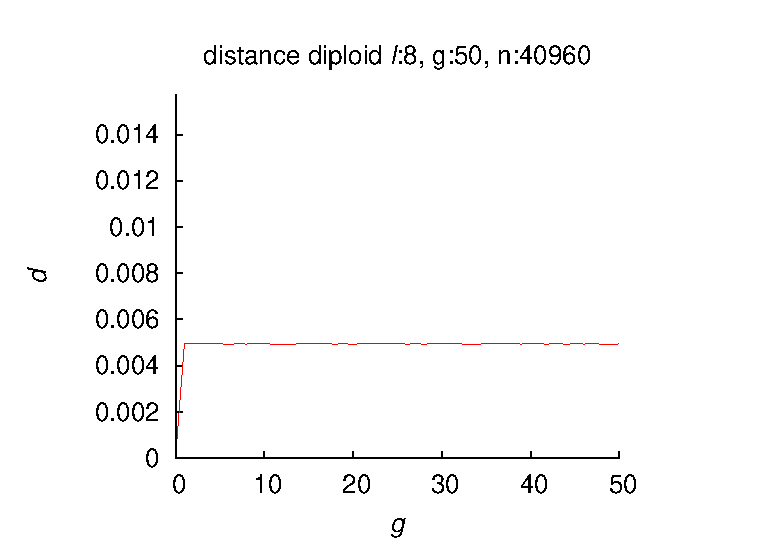
\includegraphics{figures/eps/osc/b8/n040960_osc_fin_dip_dist.eps}}}  \vspace{-1em}  \hspace{-3em}% 
\end{center}

\begin{center}
\subfloat{
\resizebox{8cm}{4.5cm}{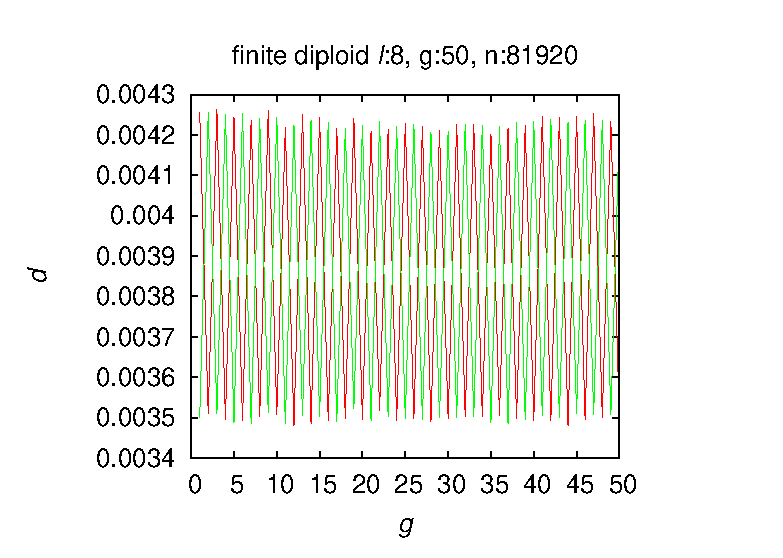
\includegraphics{figures/eps/osc/b8/n081920_osc_fin_dip.eps}}} \hspace{-3em}% 
\subfloat{
\resizebox{8cm}{4.5cm}{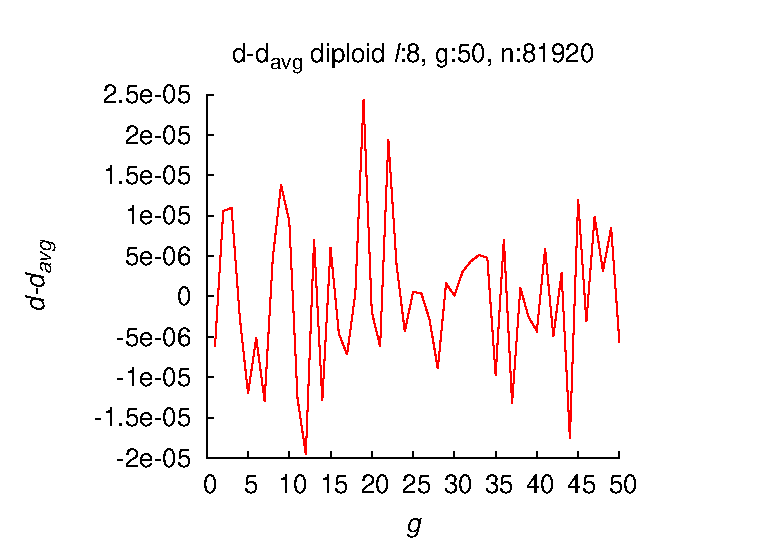
\includegraphics{figures/eps/osc/b8/n081920_osc_fin_dip_dist.eps}}}  \vspace{-1em}  \hspace{-3em}% 
\end{center}

\begin{center}
\subfloat{
\resizebox{8cm}{4.5cm}{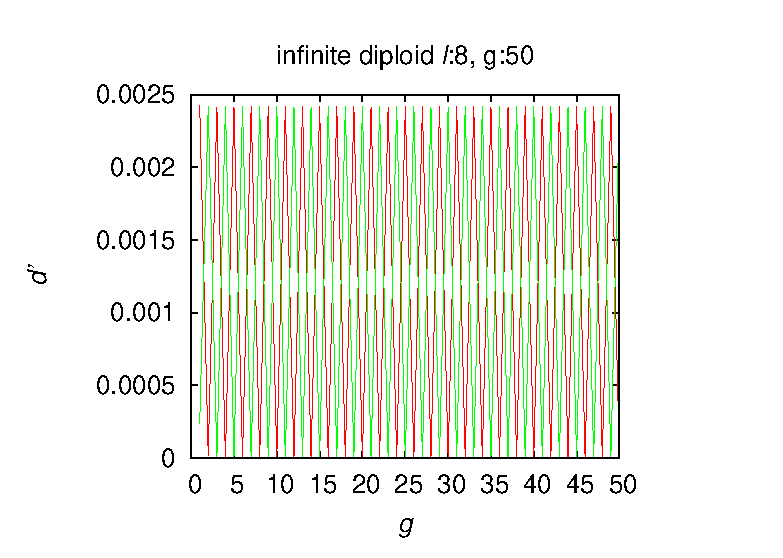
\includegraphics{figures/eps/osc/b8/osc_inf_dip.eps}}} \hspace{-3em}%
\subfloat{
\resizebox{8cm}{4.5cm}{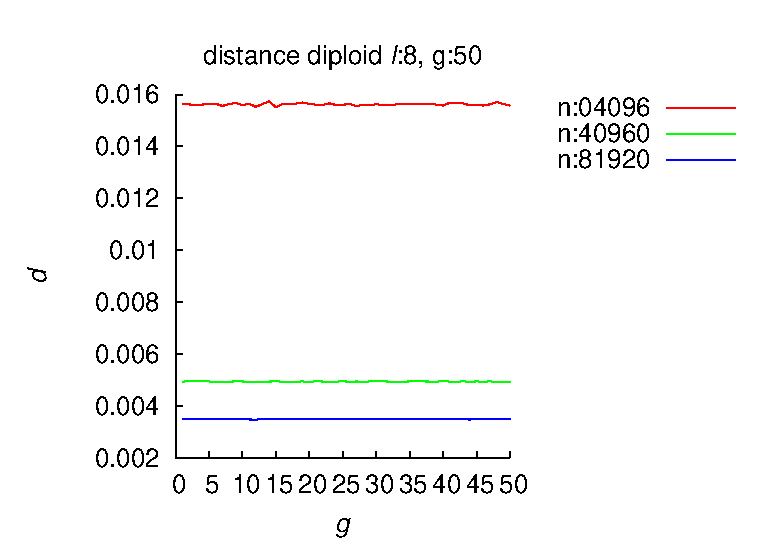
\includegraphics{figures/eps/osc/b8/fin_dip_dist.eps}}} \vspace{-0.5em} \hspace{-3em}%

\caption{\textbf{Infinite and finite diploid population oscillation behavior for genome length $\ell = 8$ (bits):} In left column, $d'$ is
  distance of finite population of size $n$ or infinite population to limits for $g$ generations. In right column, $d$ is 
  distance of finite population to infinite population for $g$ generations and $d_{avg}$ is average distance.}
\label{oscillation_8d}
\end{center}
\end{figure}

% l = 10

\begin{figure}[h]

\begin{center}
\subfloat{
\resizebox{8cm}{4.5cm}{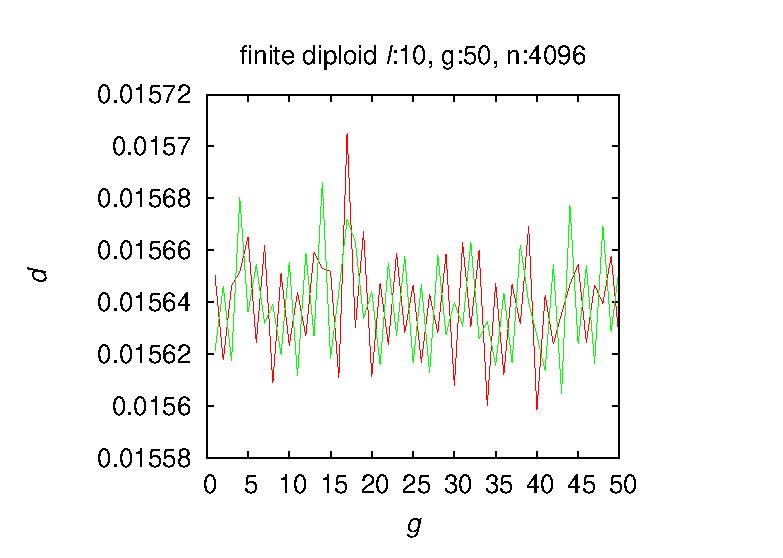
\includegraphics{figures/eps/osc/b10/n004096_osc_fin_dip.eps}}} \hspace{-3em}% 
\subfloat{
\resizebox{8cm}{4.5cm}{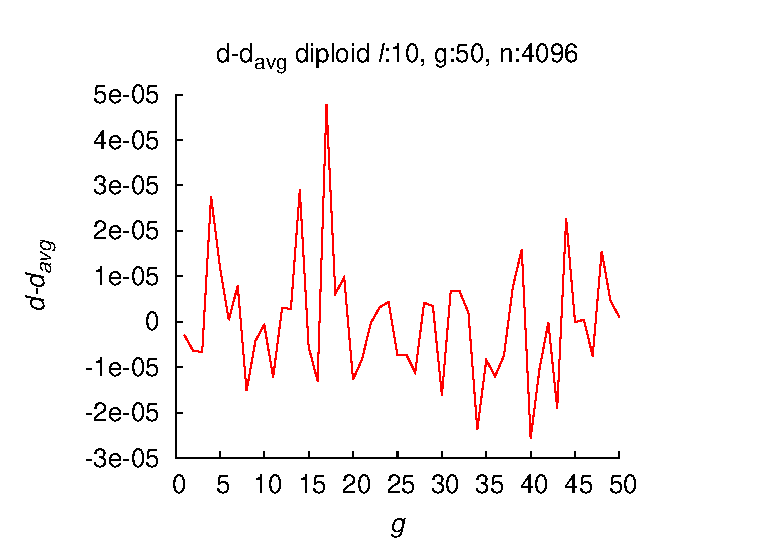
\includegraphics{figures/eps/osc/b10/n004096_osc_fin_dip_dist.eps}}}  \vspace{-1em}  \hspace{-3em}% 
\end{center}
\begin{center}
\subfloat{
\resizebox{8cm}{4.5cm}{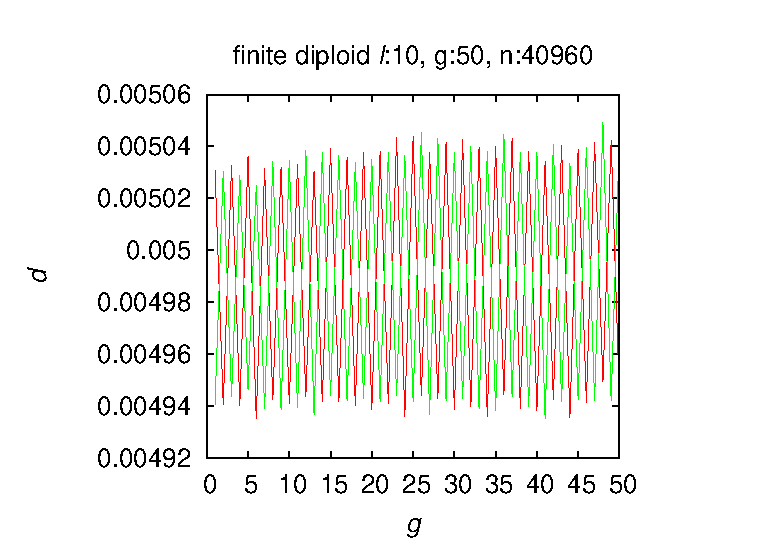
\includegraphics{figures/eps/osc/b10/n040960_osc_fin_dip.eps}}} \hspace{-3em}% 
\subfloat{
\resizebox{8cm}{4.5cm}{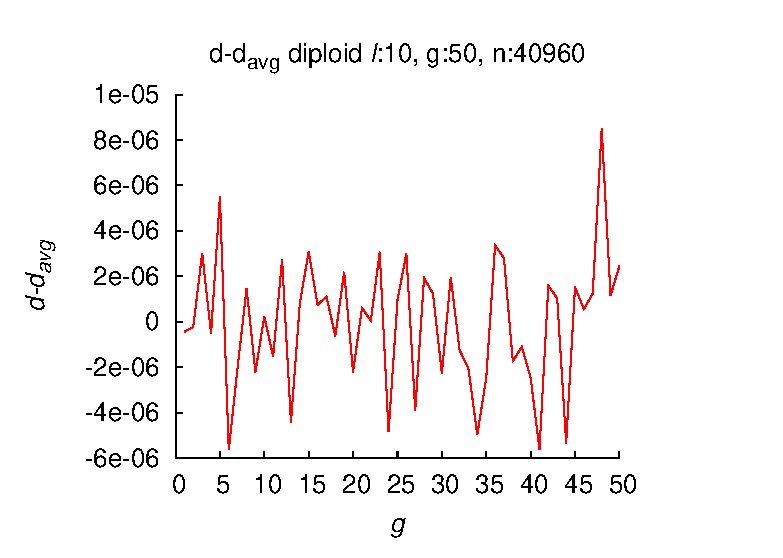
\includegraphics{figures/eps/osc/b10/n040960_osc_fin_dip_dist.eps}}}  \vspace{-1em}  \hspace{-3em}% 
\end{center}

\begin{center}
\subfloat{
\resizebox{8cm}{4.5cm}{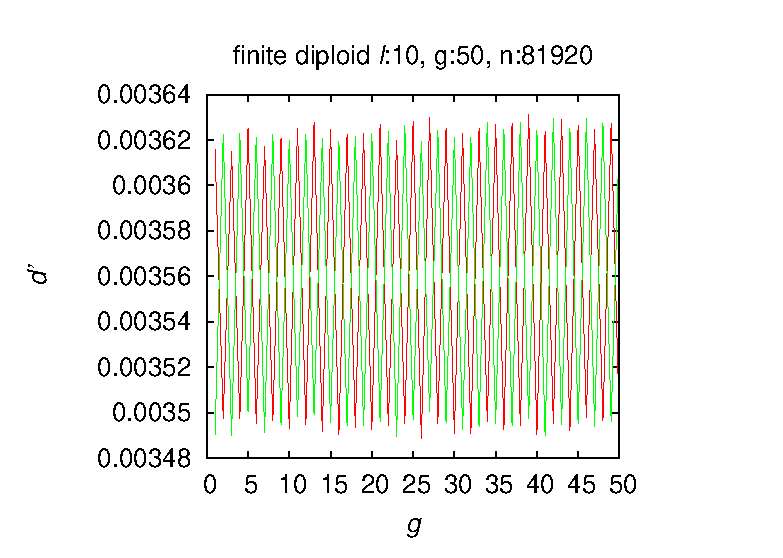
\includegraphics{figures/eps/osc/b10/n081920_osc_fin_dip.eps}}} \hspace{-3em}% 
\subfloat{
\resizebox{8cm}{4.5cm}{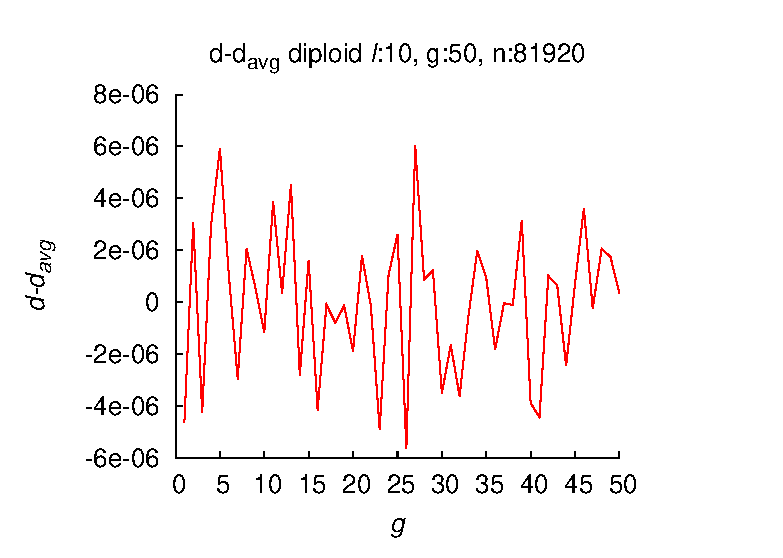
\includegraphics{figures/eps/osc/b10/n081920_osc_fin_dip_dist.eps}}}  \vspace{-1em}  \hspace{-3em}% 
\end{center}


\begin{center}
\subfloat{
\resizebox{8cm}{4.5cm}{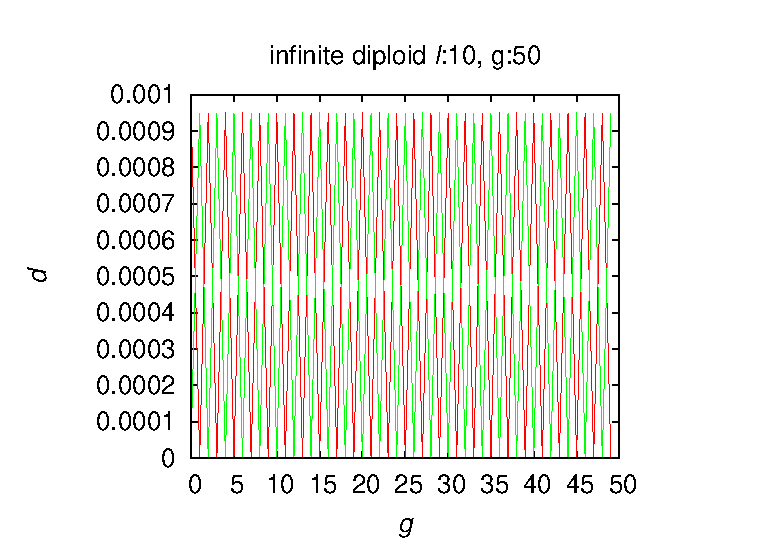
\includegraphics{figures/eps/osc/b10/osc_inf_dip.eps}}} \hspace{-3em}%
\subfloat{
\resizebox{8cm}{4.5cm}{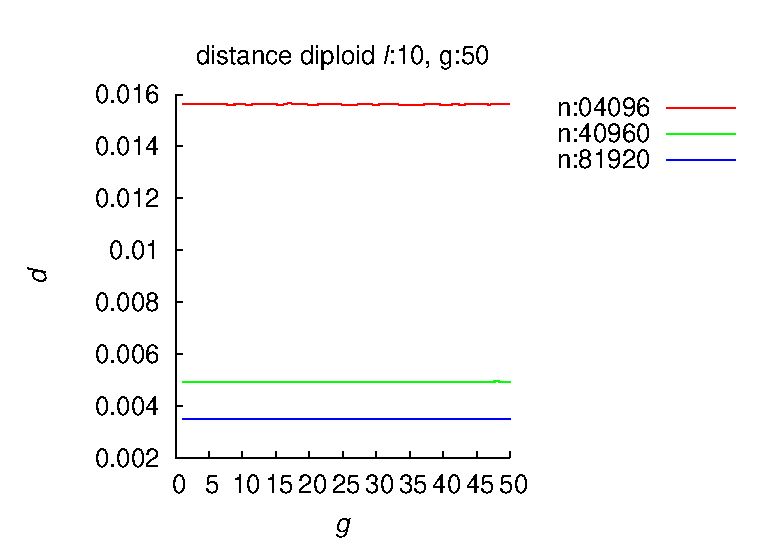
\includegraphics{figures/eps/osc/b10/fin_dip_dist.eps}}} \vspace{-0.5em} \hspace{-3em}%

\caption{\textbf{Infinite and finite diploid population oscillation behavior for genome length $\ell = 10$ (bits):} In left column, $d'$ is
  distance of finite population of size $n$ or infinite population to limits for $g$ generations. In right column, $d$ is 
  distance of finite population to infinite population for $g$ generations and $d_{avg}$ is average distance.}
\label{oscillation_10d}
\end{center}
\end{figure}

% l = 12
\begin{figure}[h]

\begin{center}
\subfloat{
\resizebox{8cm}{4.5cm}{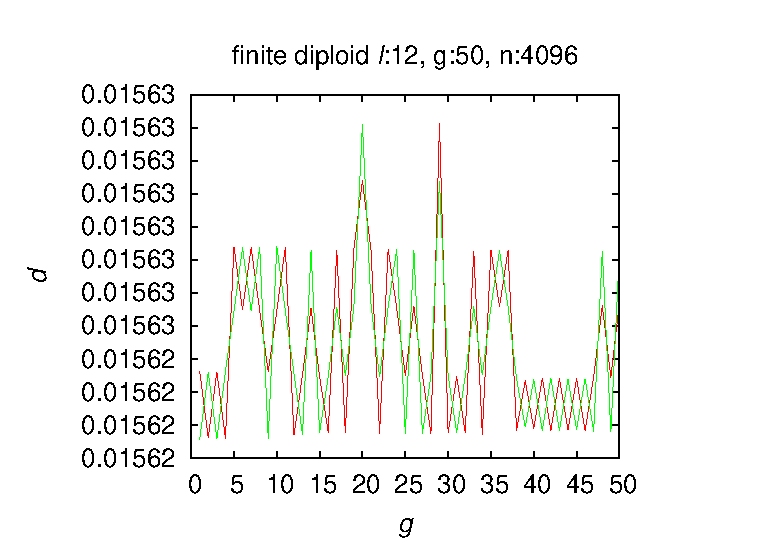
\includegraphics{figures/eps/osc/b12/n004096_osc_fin_dip.eps}}} \hspace{-3em}% 
\subfloat{
\resizebox{8cm}{4.5cm}{\includegraphics{figures/eps/osc/b12/n004096_osc_fin_dip_dist.eps}}}  \vspace{-1em}  \hspace{-3em}% 
\end{center}
\begin{center}
\subfloat{
\resizebox{8cm}{4.5cm}{\includegraphics{figures/eps/osc/b12/n040960_osc_fin_dip.eps}}} \hspace{-3em}% 
\subfloat{
\resizebox{8cm}{4.5cm}{\includegraphics{figures/eps/osc/b12/n040960_osc_fin_dip_dist.eps}}}  \vspace{-1em}  \hspace{-3em}% 
\end{center}

\begin{center}
\subfloat{
\resizebox{8cm}{4.5cm}{\includegraphics{figures/eps/osc/b12/n081920_osc_fin_dip.eps}}} \hspace{-3em}% 
\subfloat{
\resizebox{8cm}{4.5cm}{\includegraphics{figures/eps/osc/b12/n081920_osc_fin_dip_dist.eps}}}  \vspace{-1em}  \hspace{-3em}% 
\end{center}

\begin{center}
\subfloat{
\resizebox{8cm}{4.5cm}{\includegraphics{figures/eps/osc/b12/osc_inf_dip.eps}}} \hspace{-3em}%
\subfloat{
\resizebox{8cm}{4.5cm}{\includegraphics{figures/eps/osc/b12/fin_dip_dist.eps}}} \vspace{-0.5em} \hspace{-3em}%

\caption{\textbf{Infinite and finite diploid population oscillation behavior for genome length $\ell = 12$ (bits):} In left column, $d'$ is
  distance of finite population of size $n$ or infinite population to limits for $g$ generations. In right column, $d$ is 
  distance of finite population to infinite population for $g$ generations and $d_{avg}$ is average distance.}
\label{oscillation_12d}
\end{center}
\end{figure}


% l= 14
\begin{figure}[h]

\begin{center}
\subfloat{
\resizebox{8cm}{4.5cm}{\includegraphics{figures/eps/osc/b14/n004096_osc_fin_dip.eps}}} \hspace{-3em}% 
\subfloat{
\resizebox{8cm}{4.5cm}{\includegraphics{figures/eps/osc/b14/n004096_osc_fin_dip_dist.eps}}}  \vspace{-1em}  \hspace{-3em}% 
\end{center}
\begin{center}
\subfloat{
\resizebox{8cm}{4.5cm}{\includegraphics{figures/eps/osc/b14/n040960_osc_fin_dip.eps}}} \hspace{-3em}% 
\subfloat{
\resizebox{8cm}{4.5cm}{\includegraphics{figures/eps/osc/b14/n040960_osc_fin_dip_dist.eps}}}  \vspace{-1em}  \hspace{-3em}% 
\end{center}

\begin{center}
\subfloat{
\resizebox{8cm}{4.5cm}{\includegraphics{figures/eps/osc/b14/n081920_osc_fin_dip.eps}}} \hspace{-3em}% 
\subfloat{
\resizebox{8cm}{4.5cm}{\includegraphics{figures/eps/osc/b14/n081920_osc_fin_dip_dist.eps}}}  \vspace{-1em}  \hspace{-3em}% 
\end{center}

\begin{center}
\subfloat{
\resizebox{8cm}{4.5cm}{\includegraphics{figures/eps/osc/b14/osc_inf_dip.eps}}} \hspace{-3em}%
\subfloat{
\resizebox{8cm}{4.5cm}{\includegraphics{figures/eps/osc/b14/fin_dip_dist.eps}}} \vspace{-0.5em} \hspace{-3em}%

\caption{\textbf{Infinite and finite diploid population oscillation behavior for genome length $\ell = 14$ (bits):} In left column, $d'$ is
  distance of finite population of size $n$ or infinite population to limits for $g$ generations. In right column, $d$ is 
  distance of finite population to infinite population for $g$ generations and $d_{avg}$ is average distance.}
\label{oscillation_14d}
\end{center}
\end{figure}
%oscillation
\clearpage

\textbf{ Figures} \ref{oscillation_8d}, \ref{oscillation_10d}, \ref{oscillation_12d} 
and \ref{oscillation_14d} show oscillations in finite diploid populations, and distances 
between finite diploid populations and infinite diploid populations arranged by genome length $\ell$ in ascending order. 
In each figure for unique genome length $\ell$, sub-figures 
are arranged by population size $N$. In each figure, the first three rows of sub-figures in the left column show distance $d'$ of finite population 
to limits, the sub-figure in fourth row of the left column shows distance $d'$ of infinite population to limits. These sub-figures depict 
oscillating behavior of both infinite and finite diploid populations when condition \ref{OscCond} is met. 
Like in haploid population case, as population size increases, oscillation approaches the behavior exhibited by infinite population. 

In each figure (\ref{oscillation_8d}, \ref{oscillation_10d}, \ref{oscillation_12d}, 
and \ref{oscillation_14d}), the first three graphs in the right column show 
distance variation (difference of distance $d$ and average distance $d_{avg}$)  
where $d$ is distance between diploid finite and infinite populations and $d_{avg}$ is average value of $d$. 
The graph in the fourth row of the right column combines distance plots between finite and infinite populations for sizes 
($N = N_0^2, \nudge10N_0^2, \nudge20N_0^2$). The graphs show distance decreases 
as population size increases, consistent with results from section \ref{convergence}. 
The graphs of $d-d_{avg}$ decrease in amplitude as population size increases. 
For fixed finite population size, as $\ell$ increases, the distance graphs become smoother, and amplitude of oscillations decrease.

Distance data obtained from simulations for diploid populations are summarized in table \ref{tableDistanceOscDip}, 
which tabulates average distance between finite and infinite populations 
for population sizes $N \;=\; 4096 $, $N \;=\; 40960 $ and $N \;=\; 81920 $.
%
\begin{table}[h]
\caption[\textbf{Distance measured for diploid population}]{\textbf{Distance measured for diploid population:} $N$ is population size, $\ell$ is genome length, 
average distance between finite and infinite population is tabulated in the last three columns, and last row is expected single step distance.}
\centering
\begin{tabularx}{0.75\textwidth}{ c *{3}{X}}
\toprule
$\ell$ & $N \;=\; 4096 $ & $N \;=\; 40960 $ & $N \;=\; 81920 $\\
\midrule
8 & 0.0156 & 0.0049 & 0.0035 \\
10 & 0.0156 & 0.0049 & 0.0035 \\
12 & 0.0156 & 0.0049 & 0.0035 \\
14 & 0.0156 & 0.0049 & 0.0035 \\
\midrule
$1/\sqrt{N}$ & 0.0156 & 0.0049 & 0.0035 \\
\bottomrule

\end{tabularx}
\label{tableDistanceOscDip}
\end{table}

Results from table \ref{tableDistanceOscDip} show average distance between finite and infinite population closely follows 
the expected single step distance. The distance decreases as $1/\sqrt{N}$.

\section{Discussion}
For same genome length $\ell$ and same size finite populations, graph showing distance between finite diploid population and infinite population is 
smoother than graph showing distance between finite haploid population and infinite population. Average oscillation amplitude is 
plotted for both haploid and diploid populations as surface graphs in figures \ref{fig:osc_amp_hap} and \ref{fig:osc_amp_dip}.

\begin{figure}[h]
\begin{center}
\subfloat[]{\label{fig:osc_amp_hap}
\resizebox{7.5cm}{5cm}{\includegraphics{figures/eps/osc/osc_amp_hap.eps}}} %
\subfloat[]{\label{fig:osc_amp_dip}
\resizebox{7.5cm}{5cm}{\includegraphics{figures/eps/osc/osc_amp_dip.eps}}} \vspace{-0.5em} %

\caption[\textbf{Average oscillation amplitude}]{\textbf{Average oscillation amplitude:} $A$ is average amplitude of oscillation, $L$ is genome length $\ell$, and $N$ is population size}
\label{osc_amp}
\end{center}
\end{figure}

Oscillation amplitude increases with increase in population size for both haploid and diploid populations, 
and better oscillations are observed with larger population size for a given $\ell$. 
Also amplitude of oscillation decreases with increase in $\ell$ value for same population size, 
and since total genome length of diploid population is twice that of haploid population, 
amplitude of oscillation of diploid population is smaller than haploid population of same population size and same value of $\ell$. 
So for longer genome length $\ell$, larger population size is needed to observe clear oscillations.

\begin{figure}[h]
\begin{center}
\subfloat[]{\label{fig:osc_12d_N4096}
\resizebox{7.5cm}{5cm}{\includegraphics{figures/eps/osc/b12/b12_n004096_osc_fin_dip_lvl.eps}}} 
\subfloat[]{\label{fig:osc_14d_N4096}
\resizebox{7.5cm}{5cm}{\includegraphics{figures/eps/osc/b14/b14_n004096_osc_fin_dip_lvl.eps}}} \vspace{-0.5em} 

\caption{\textbf{Finite diploid population oscillation for $\ell = 12 \;\&\; 14$ and $N = 4096$}}
\label{oscillation_12d_14d_N4096}
\end{center}
\end{figure}

For the diploid case, when genome length $\ell$ is longer ($\ell$ = 12 and 14 in our simulation), 
and population size is small (like N = 4096 in our simulation), finite population has tendency to 
jump between different levels. Figures \ref{fig:osc_12d_N4096} and \ref{fig:osc_14d_N4096} show such tendency for 
$\ell$ = 12 and $\ell$ = 14. Very good oscillations with tiny amplitude were observed in temporarily stable states 
in these cases. Figure \ref{oscillation_14d_N4096} shows magnified scale oscillations for $\ell \;=\; 14$ 
when high peak is omitted from the plot of \ref{fig:osc_14d_N4096}. 
As string length increases, the number of fixed points also increases, 
and finite populations tend to stay near fixed points(see \cite{Vose1999}). With many fixed points available, 
there are several regions for finite populations to prefer. 
But when population size is large, finite populations intend to follow the infinite population, 
and infinite population tends to 
converge to a single fixed point or oscillate between two fixed points, and thus, 
larger populations have lower tendency to jump between different levels.
\clearpage

\begin{figure}[htp]
\begin{center}
\subfloat{
\resizebox{8cm}{5cm}{\includegraphics{figures/eps/osc/b14/b14_n004096_osc_fin_dip_10_50.eps}}} \hspace{-3em}%
\caption{\textbf{Finite diploid population oscillation for $\ell = 14$ and $N = 4096$ from 10 to 50 generations}}
\label{oscillation_14d_N4096}
\end{center}
\end{figure}


\section{Summary}
In this chapter, we described infinite population limits predicted by Vose, and conditions 
for convergence to periodic orbits. Mutation distributions and crossover distributions were computed 
to satisfy the conditions for infinite populations to converge to periodic orbits. Through experiment, 
we showed finite populations can also exhibit approximate oscillation. 
We found amplitude of oscillation is affected by string length used and population size. 
As string length increases, oscillation amplitude decreases. 
As population size increases, oscillation amplitude increases and also randomness in oscillation decreases. 
Simulations show finite populations with smaller population size and higher string length may oscillate 
between different pairs of fixed points, which occurred in diploid populations only in our simulations. 
Moreover, the distance between finite populations and infinite populations can in practice decrease 
as $1/\sqrt{N}$ as the populations size increases, which is in agreement with previous results from 
chapter 2.





 
